This section will explain the basic theory and concept behind Ambient Occlusion. The section will end with an explanation of how the math behind the technique is derived.

\subsection{The Basic Concept}
Ambient Occlusion works by seeing how much of an external envirornment can be seen from each surface point on the object to be rendered. The more of the external envirornment that can be seen the more ambient lighting that point will recieve. This type of illumination is therefore often called "sky light" in production because it simulates how a model would be lighted on an overcast day since the light from ambient occlusion is incident on the point from all directions.
\\ \\
When ambient occlusion is calculated two factors are calculated. The first is the accessibility term and this is the measure of how much of the envirornment that is accessible from the surface point. The other is the "bent normal" which is the average direction of the incident light from the envirornment. The bent normal can then be used to look up into an envirornment map in order to give more realistic lighting without the added cost of a global illumination algorithm.
\subsection{Mathemathical Foundation}
Ambient Occlusion as all other realistic rendering methods tries to approximate the rendering equation:
\[ 
L_o(\textbf{x},\overrightarrow{w}) = 
L_e(\textbf{x},\overrightarrow{w}) +
\int_{2\pi}
 f_r(\textbf{x},\overrightarrow{w}',\overrightarrow{w} )L_i(\textbf{x},\overrightarrow{w}')\cos\theta dw'
\]
We will aproximate this with the Monte Carlo estimator:
\[ 
L_o(\textbf{x},\overrightarrow{w}) = 
L_e(\textbf{x},\overrightarrow{w}) +
\frac{1}{N}
\sum_{i=1}^N \frac{ 
 f_r(\textbf{x},\overrightarrow{w}',\overrightarrow{w} )L_i(\textbf{x},\overrightarrow{w}')\cos\theta
}
{
pdf(\overrightarrow{w}_i')
}
\]
if we only consider diffuse reflectance then the BRDF is equal to the BRDF for Lambertian reflectance:
\[
 f_r(\textbf{x},\overrightarrow{w}',\overrightarrow{w}) = \frac{R_d}{\pi}
\]
Then the expression becomes:
\[ 
L_o(\textbf{x},\overrightarrow{w}) = 
L_e(\textbf{x},\overrightarrow{w}) +
\int_{2\pi} \frac{ 
\frac{R_d}{\pi})L_i(\textbf{x},\overrightarrow{w}')\cos\theta dw'
}
{
pdf(\overrightarrow{w}_i')
}
\]
A good probability density function would therefore be:
\[
pdf((\overrightarrow{w}_i')) = cos\theta / \pi
\]
The goal is therefore to find a sampling method that has this probability density function. One is:
\[
\overrightarrow{w}_i' = (\theta,\phi) =
(\cos^{-1}\sqrt{r_1},2\pi r_2)
\]
Where r1 and r2 is random numbers between 0 and 1.
When this sampling method is used and a visibility function denoted V is used to describe incident illumination the equation finaly becomes
\[ 
L_o(\textbf{x},\overrightarrow{w}) = 
\frac{R_d}{N} \sum_{i=1}^N V(\overrightarrow{w}_i')
\]
Where V is equal to 1 if the direction is unoccluded and 0 otherwise. In a raytracer this is normally done by casting N rays with origin in the surface point being sampled with a random direction in the point's hemisphere and divide the result by N. These
\subsection{Disadvantages}
The main problem with Ambient Occlusion is from the fact that it reduces the problem of finding incident light to using the calculated bent normal to do a texture lookup in an envirornment map. Since the bent normal is the average direction of incident light it can in certain cases point in a direction that is actually occluded as illustrated by figure:
\\
\begin{figure}[h]
	\centering
	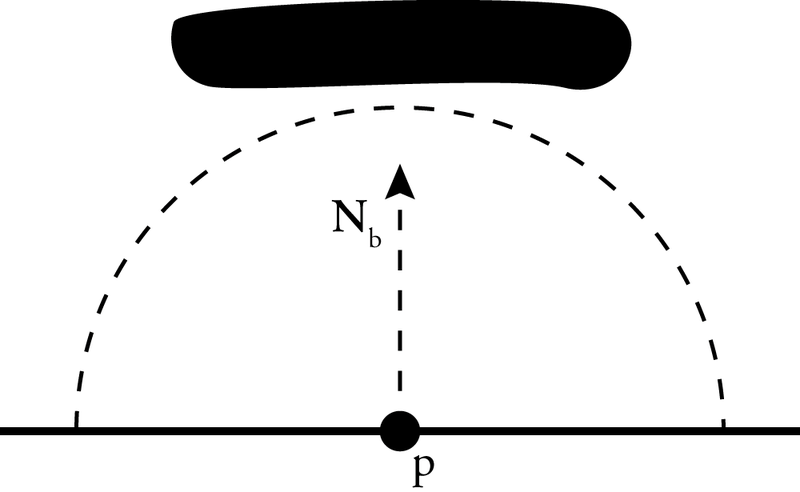
\includegraphics[width=0.6\textwidth]{Theory/bentNormalProblems}
	\label{fig:bent_normal}
	\caption{The problem of using a bent normal Nb to find the irradiance at point P.}
\end{figure}
\\
However since ambient occlusion is used to calculate the diffuse terms

\subsection{Envirornment maps}

\subsection{High Dynamic Range Imaging}

The next section will cover our implementation of Ambient Occlusion.
